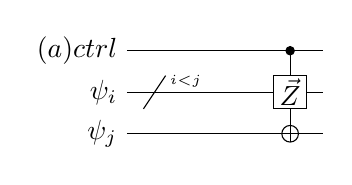
\begin{tikzpicture}[scale=1.000000,x=1pt,y=1pt]
\filldraw[color=white] (0.000000, -7.500000) rectangle (71.000000, 37.500000);
% Drawing wires
% Line 1: a W \text{(a) }ctrl
\draw[color=black] (0.000000,30.000000) -- (71.000000,30.000000);
\draw[color=black] (0.000000,30.000000) node[left] {$\text{(a) }ctrl$};
% Line 2: b W \psi_i
\draw[color=black] (0.000000,15.000000) -- (71.000000,15.000000);
\draw[color=black] (0.000000,15.000000) node[left] {$\psi_i$};
% Line 3: c W \psi_j
\draw[color=black] (0.000000,0.000000) -- (71.000000,0.000000);
\draw[color=black] (0.000000,0.000000) node[left] {$\psi_j$};
% Done with wires; drawing gates
% Line 5: b / ^{i<j}
\draw (6.000000, 9.000000) -- (14.000000, 21.000000);
\draw (12.000000, 18.000000) node[right] {$\scriptstyle{^{i<j}}$};
% Line 6: a b c LABEL
% Line 7: b G $\vec{Z}$ a +c
\draw (59.000000,30.000000) -- (59.000000,0.000000);
\begin{scope}
\draw[fill=white] (59.000000, 15.000000) +(-45.000000:8.485281pt and 8.485281pt) -- +(45.000000:8.485281pt and 8.485281pt) -- +(135.000000:8.485281pt and 8.485281pt) -- +(225.000000:8.485281pt and 8.485281pt) -- cycle;
\clip (59.000000, 15.000000) +(-45.000000:8.485281pt and 8.485281pt) -- +(45.000000:8.485281pt and 8.485281pt) -- +(135.000000:8.485281pt and 8.485281pt) -- +(225.000000:8.485281pt and 8.485281pt) -- cycle;
\draw (59.000000, 15.000000) node {$\vec{Z}$};
\end{scope}
\filldraw (59.000000, 30.000000) circle(1.500000pt);
\begin{scope}
\draw[fill=white] (59.000000, 0.000000) circle(3.000000pt);
\clip (59.000000, 0.000000) circle(3.000000pt);
\draw (56.000000, 0.000000) -- (62.000000, 0.000000);
\draw (59.000000, -3.000000) -- (59.000000, 3.000000);
\end{scope}
% Done with gates; drawing ending labels
% Done with ending labels; drawing cut lines and comments
% Done with comments
\end{tikzpicture}
